\section{Himpunan}
Hanya review, harusnya sejak SMP sudah paham mengenai himpunan / \textit{set} :).

Misalkan $A$ dan $B$ adalah dua himpunan.
\begin{enumerate}
    \item $\phi$ atau $\{\}$ adalah himpunan kosong atau himpunan yang tidak mempunyai elemen.
    \item Banyak elemen dari $A$ dinotasikan dengan $|A|$ (dibaca "kardinalitas dari $A$") atau $n(A)$ .
    \item $x \in A$ dibaca $x$ elemen dari $A$.
    \item $A \subseteq B$ dibaca $A$ subset dari $B$ atau $A$ himpunan bagian dari $B$.
    \item $A \subset B$ dibaca $A$ adalah proper subset dari $B$. Bedanya dengan $\subseteq$?\\
    $\subset$ itu mirip $<$ dimana tidak mungkin $A \subset A$, tetapi $\subseteq$ itu mirip $\le$ karena mungkin $A \subseteq A$.
    \item $A \cup B$ dibaca $A$ union $B$ atau $A$ gabung $B$.
    \item $A \cap B$ dibaca $A$ intersection $B$ atau $A$ irisan $B$.
    \item $A^c$ atau $A'$ dibaca $A$ komplemen.
    \item $|A \cup B| = |A|+|B|-|A \cap B|$.
\end{enumerate}
	
\subsection{Himpunan Bilangan-bilangan}
\begin{figure}[h]
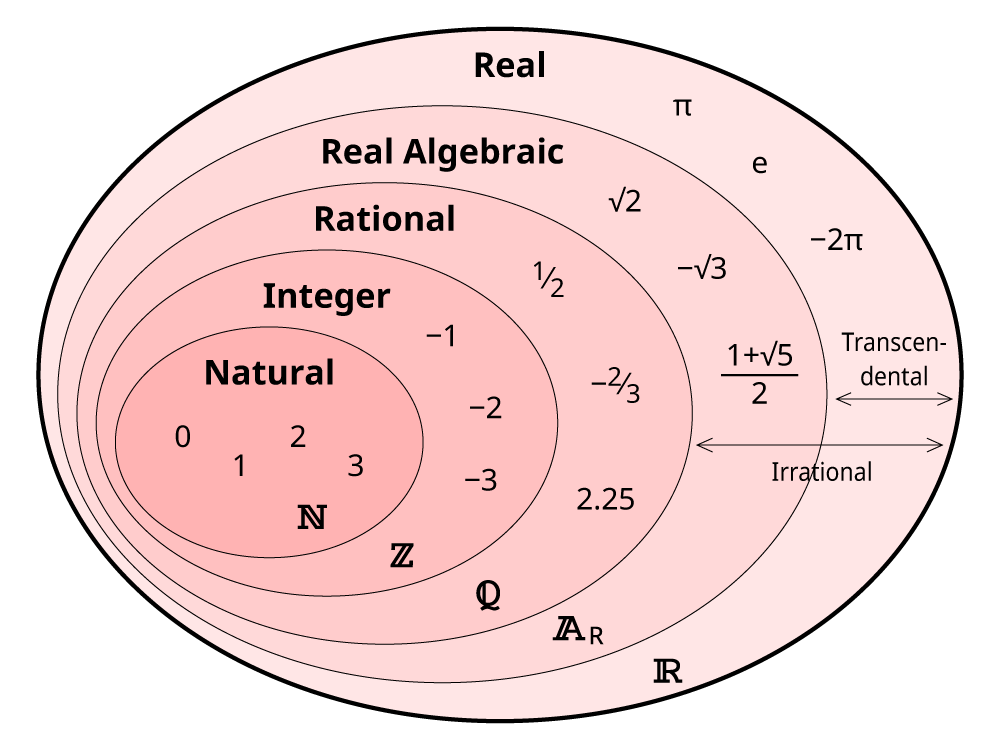
\includegraphics[width=\textwidth/2]{High/numbers set.png}
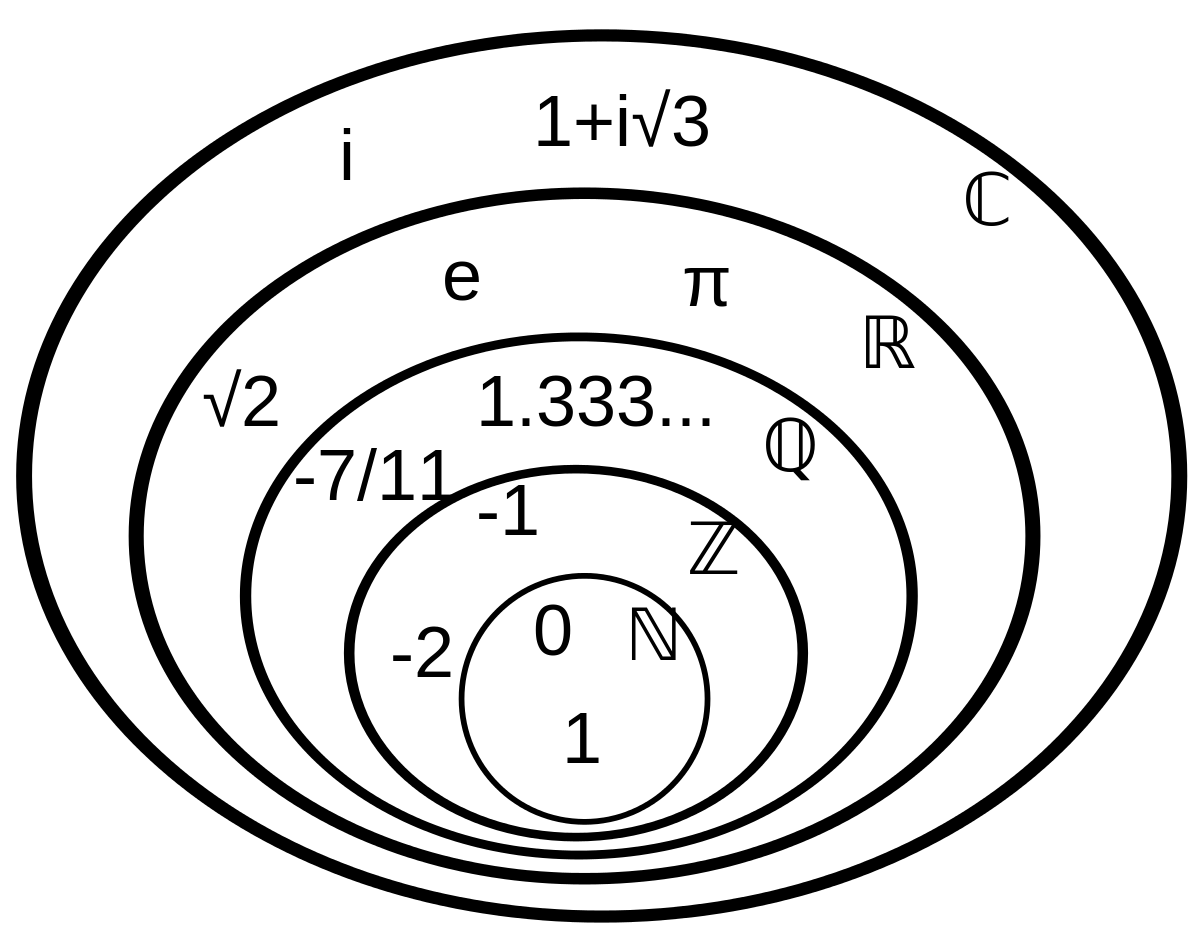
\includegraphics[width=\textwidth/2]{High/compset.png}
\caption{dari: https://thinkzone.wlonk.com/Numbers/RealSet\_w1000.png}
\caption{dan https://en.wikipedia.org/wiki/Number}
\end{figure}

\begin{enumerate}
\item $\NN$ adalah himpunan bilangan asli (Natural Numbers) $\{1,2,3,\dots\}$. Di beberapa negara Eropa dan beberapa negara lain, himpunan bilangan asli adalah $\{0,1,2,\dots\}$.
\item $\ZZ$ adalah himpunan bilangan bulat $\ZZ=\{\dots,-2,-1,0,1,2,\dots\}$.
\item $\QQ$ adalah himpunan bilangan rasional, dengan definisi $\QQ=\{\dfrac{a}{b}\mid a\in \ZZ, b\in\ZZ^+\}$.
\item $\RR$ adalah himpunan bilangan real, semua bilangan yang ada di dunia nyata, termasuk bilangan irasional seperti $\sqrt{2}$ dan rasional.
\item $\CC$ adalah himpunan bilangan kompleks dengan definisi\\ $\CC = \{a+bi \mid a,b \in \RR \text{ dan }i=\sqrt{-1}\}$.
\item Definisikan pula $\ZZ^+$ sebagai himpunan bialangan bulat positif. Aturan yang sama juga berlaku: $\RR^+, \QQ^+$.
\end{enumerate}